%% ------------------------------------------------------------------------- %%
\chapter{Introdução}
\label{cap:introducao}

\begin{section}{Motivação}

Os avanços nos campos tecnológicos e computacionais levaram uma enorme expansão
dos ecossistemas de \textit{software}. Novos programas são criados para
suprir as necessidades dos mais diversos domínios, seja através de sistemas web
codificados em linguagens de \textit{script}; ou por componentes para
sistemas operacionais destinados a embarcados, com a finalidade de controlar algum
recurso do \textit{hardware}. Independente da razão por trás do desenvolvimento
do \textit{software}, é certo que, em alguma etapa, seu código será transformado em linguagem
de máquina por um compilador, mesmo que ele seja executado por um
interpretador.

Um compilador nada mais é que um \textit{software} que traduz um código em uma linguagem
de programação $A$ para outra linguagem $B$ \citep{dragonbook}.  Compiladores
são programas enormes, largamente adotados pela indústria e academia, onde muito
esforço e pesquisa foi e ainda é empregado para que eles produzam código
eficiente, com destaque para a corretude. Existem projetos enormes destinados a desenvolvê-los e
aprimorá-los, como o Gnu Compiler Collection
(GCC\footnote{https://gcc.gnu.org/}), capaz de traduzir diversas linguagens
como C, C++ e Fortran, para linguagem de máquina. Há também outros projetos
menores como o F2C\footnote{https://www.netlib.org/f2c/}, um compilador de
Fortran para C, utilizado em ambientes onde não há um compilador Fortran
disponível.

Embora seja possível escrever código em linguagem de máquina, o que
tornaria um compilador desnecessário, isto é extremamente caro e
sujeito a erros, além de ser uma prática extremamente
incomum nos projetos contemporâneos a este trabalho \citep{githuboctoverse} (vide
Figura \ref{fig:github_2017}). Escrever programas em código de máquina tende a
ser trabalhoso e financeiramente custoso, com difícil manutenção e quase impossível portabilidade.
Um exemplo disso é o \textit{Internal Revenue Service} (IRS) dos Estados Unidos,
que ainda mantém máquinas compatíveis com o IBM System/360 devido a existência no sistema
de várias linhas de código escritas em linguagem de montagem para essa
arquitetura \citep{gao}. Esse problema ganhou visibilidade na imprensa após a falha no
\textit{Tax Day} de 2018 \citep{tax_failure}.

Compiladores são usados em projetos dos mais variados tamanhos.
Grandes projetos podem conter milhões de linhas de código, e até mesmo
construir novas linguagens para facilitar o desenvolvimento de novas
funcionalidades, e portanto o processo de compilação precisa ser rápido
para viabilizar o seu desenvolvimento. Logo, muito estudo é aplicado
para desenvolver algoritmos mais eficientes para eles, além de técnicas
de computação paralela para aproveitar os recursos dos processadores
\textit{multicore}, cada vez mais comuns.

%TODO: Deixar essa imagem mais legível
\begin{figure}[ht]
 \centering
 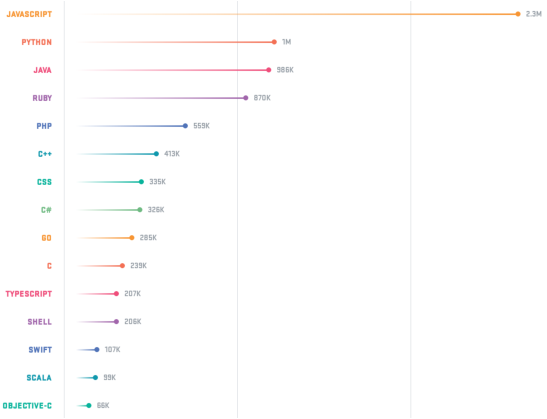
\includegraphics[scale=1.8]{github_2017.pdf}
 \caption{As 15 linguagens mais usadas no GitHub em 2017. Fonte: \cite{githuboctoverse}}
 \label{fig:github_2017}
\end{figure}

\end{section}

\begin{section}{O GCC}

O GCC é um compilador de código aberto amplamente usado tanto no meio
acadêmico quanto na indústria. Por ser um grande projeto, o GCC contém uma
linguagem própria para facilitar a adição de otimizações na geração de
código, que em seguida é compilado em um único arquivo C, para (1)
aproveitar as otimizações já implementadas no próprio compilador, e (2)
evitar reescrever várias funcionalidades já implementadas. Infelizmente, este processo
gera um gargalo na compilação do projeto em máquinas \textit{manycore}, pois o
GCC não é capaz de compilar um arquivo em paralelo de maneira incremental.

Atualmente, todo o paralelismo na fase de compilação é provido pelo GCC de
duas maneiras distintas: ou pelo GNU Make\footnote{https://www.gnu.org/software/make/},
que apenas fornece uma granularidade a nível dos arquivos; ou através da estrutura do
LTO, que será abordada na Seção \ref{chap:related_works}. Esse gargalo pode parecer uma
característica peculiar do projeto GCC, mas discussões com a comunidade levaram
usuários a relatar o mesmo problema em seus projetos. Tal problema pode ser
mitigado por um compilador que seja capaz de compilar um único arquivo em paralelo
\citep{mailgcc} \citep{phoronix}.  Outra possível solução seria
partir o arquivo em arquivos menores e utilizar o esquema de
paralelismo já existente do GNU Make, mas isto implica em uma modificação na
estrutura do projeto, o que pode não ser o ideal.

Considerando que atualmente há uma tendência para que os processadores sejam
cada vez mais paralelos, compiladores que usufruam deste recurso poderiam
reduzir o tempo de compilação de um projeto, ou de uma suíte de testes que
necessita recompilação antes de sua execução, economizando recursos no caso da
computação ser cobrada por hora. Até então, o paralelismo empregado internamente
em compiladores otimizadores foi consequência de uma estrutura criada para
permitir otimizações mais agressivas e custosas, como o LTO
\citep{glek2010optimizing}.

\end{section}

\begin{section}{Questões de Pesquisa}

Deve ser observado que nem todos os processos de um compilador podem ser
paralelizados. Compiladores operam em etapas que podem ser fortemente
dependentes do resultado da etapa anterior. Por exemplo, ao compilar uma
função em C, pode ser necessário saber se alguma outra foi declarada anteriormente; ou
então o analisador sintático pode alterar um estado do analisador léxico para
detectar variáveis de um novo tipo. Além disto, compiladores também se apoiam em algoritmos
em grafos, cujo paralelismo é um desafio \citep{lumsdaine2007challenges}.

% TODO: Deixar as questões de pesquisa mais detalhadas, e talvez colocar em outra
% subseção.
Sendo assim, esse trabalho concentra-se em duas questões de pesquisas:
\begin{description}
    \item[\textit{QP1}] - Em que pontos um compilador pode usufruir de paralelismo?

    \item[\textit{QP2}] - Qual é o ganho de desempenho ao paralelizar internamente um compilador?
\end{description}
essas questões de pesquisa visam propor uma alternativa ao LTO com foco
em desenvolvimento incremental, e também cobrindo os casos onde o LTO produz binários menos
eficientes através de melhorias no paralelismo do processo clássico de compilação.
Para validar os resultados, este trabalho inclui a implementação no GCC de algumas das
técnicas discutidas, além da utilização de técnicas de inferência estatística para
análises no tempo total de compilação no projeto GCC e arquivos separados.

Este trabalho está dividido nos seguintes capítulos: no Capítulo
\ref{chap:fundamentacao}, são apresentados conceitos teóricos como parte da
Teoria de Compiladores e Computação Paralela para que seja possível
compreender as questões acerca do trabalho.  Em sequência, o Capítulo
\ref{chap:related_works} contém uma apresentação dos trabalhos relacionados
a paralelismo de compiladores até o estado da
arte nesse tópico, além de uma breve discussão sobre seus pontos positivos
e negativos. Por fim, o Capítulo \ref{chap:proposta} apresenta uma visão geral
do trabalho de fato, com uma análise de tempo consumido que permitiu
identificar quais pontos necessitam de melhorias, além da
proposta do trabalho, que contempla a arquitetura de paralelismo e o
planejamento de sua implementação.



\end{section}
